\chapter{Proposta de Trabalho}\label{chap:proposta}

\section{Motivação e Objetivo}

No Capítulo~\ref{chap:revisao} foram apresentados os métodos
que buscam modificar os conjuntos de dados para torná-los
mais representativos para o problema em estudo.  Discutiu-se
que os métodos automáticos impedem que os usuários orientem
essas modificações e ao mesmo tempo imponham seus
conhecimentos sobre os resultados.  Apresentou-se as
ferramentas visuais que surgem como uma interessante
alternativa aos métodos automáticos, pois permitem a
interação dos usuários, mas que ainda apresentam certas
limitações em relação às interfaces utilizadas e aos
mecanismos de interação propostos.

O uso de ferramentas visuais que operam sobre grandes
volumes de dados não é exclusivo aos trabalhos relacionados
ao aqui proposto. Na verdade, toda a área de
Mineração Visual de Dados~\cite{Wong1999} (MVD),
\emph{Visual Data Mining}, tem como objetivo justamente
envolver os usuários em tarefas que até então eram
executadas de maneira totalmente automática. A principal
motivação desta área parte do princípio de quando o usuário
consegue compreender o resultado apresentado por uma
representação visual, ele confia neste resultado e
consegue obter melhor proveito das análises~\cite{Wong1999}.

Uma característica fundamental para ferramentas MVD é manter
a simplicidade em todos aspectos do sistema~\cite{Wong1999}.
No entanto, muitas das ferramentas discutidas anteriormente
se baseiam em interfaces demasiadamente complexas, as quais
exigem do usuário um certo período de treinamento para um
uso efetivo. Tendo em vista que o objetivo das ferramentas
visuais é tornar as análises mais intuitivas, qualquer tipo
de obstáculo, como a necessidade de treinamento do usuário,
pode ser desfavorável ao se comparar com os métodos
automáticos.

Um outro aspecto que deve ser levado em consideração para o
desenvolvimento dessas ferramentas é permitir seu uso em
diversos domínios~\cite{Wong1999}. Para isso, diferentes
mecanismos de interação devem ser oferecidos, já que nenhum
será capaz de operar otimamente para todas as
aplicações. Porém, unir em um único ambiente os principais
mecanismos necessários para a modificação efetiva dos dados
não é tarefa trivial e nenhum dos trabalhos estudados provê
tal funcionalidade.

Uma questão que deve ser considerada em ferramentas de
exploração de dados, sejam elas visuais ou não, é
possibilitar investigações em subconjuntos dos dados. Isto é
importante pois dificilmente o conjunto de dados apresentará
um comportamento global, sendo mais provável que existam
subconjuntos com diferentes características que devem ser
avaliadas localmente~\cite{May2011}. Porém, poucos dos
trabalhos estudados atentam para esta questão.

Levando em consideração os aspectos mencionados nos
parágrafos acima: simplicidade da ferramenta, diversidade
dos mecanismos de interação e avaliação global e local dos
dados, este projeto de mestrado se baseia no uso de
\emph{Biplots}~\cite{Gabriel1971} para desenvolver uma
abordagem que apresente essas características e que seja
capaz de superar as limitações dos trabalhos do atual estado
da arte.

O estabelecimento de \emph{biplots} como base para este trabalho é
adequado, pois biplots oferecem uma representação simultânea
entre itens e dimensões de forma simples. A
Figura~\ref{fig:biplot} apresenta um exemplo de biplot para
os dados da Tabela~\ref{tab:at}.
Neste exemplo, os pontos representam os países e as setas
representam os aspectos avaliados no levantamento. A
distância entre os pontos é relacionada com a similaridade
entre os países, de modo que pontos que se encontram
próximos indicam países com características em comum. O
mesmo pode ser dito em relação às setas, de modo que setas
com mesma direção simbolizam atributos correlacionados. Além
disso, o comprimento das setas é proporcional ao desvio
padrão das variáveis que representam.

\begin{figure}[h!]
    \centering
    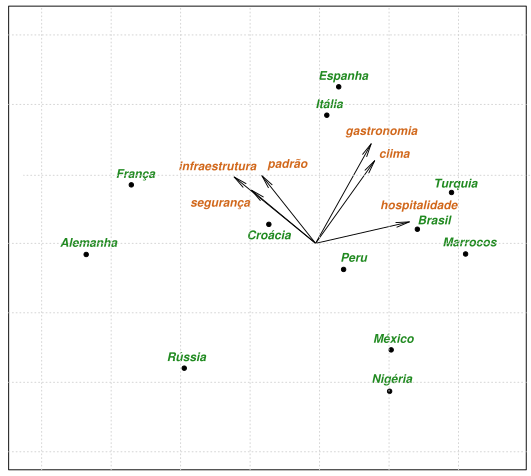
\includegraphics[width=10cm]{images/biplot.pdf}
    \caption{Exemplo de biplot para os dados da
    Tabela~\ref{tab:at}.}
    \label{fig:biplot}
\end{figure}

Poucas técnicas visuais são capazes de apresentar
simultaneamente informações sobre itens e dimensões em uma
única representação. Mesmo entre a minoria que apresenta
essa característica, nenhuma é capaz de estabelecer uma
coerência entre as duas representações e essa é uma
propriedade de biplots que os tornam ferramentas únicas. Tal
propriedade pode ser observada na Figura~\ref{fig:biplot},
onde nota-se, por exemplo, que o Brasil se encontra naquela
posição do espaço, pois é um país com excelente
hospitalidade, clima agradável e boa comida. 

Essas características de biplots fazem com que seu uso seja
propício para a construção de ferramentas interativas de
transformação de dados multidimensionais. No entanto,
desconhece-se qualquer trabalho na literatura que faça uso
de tal representação gráfica para transformar
interativamente conjuntos de dados. Assim, acredita-se que
mesmo os mecanismos interativos que já foram utilizados em
outros trabalhos, como os de redução de dimensionalidade
interativa, apresentarão características únicas na
metodologia aqui proposta.

De um modo geral, o objetivo deste trabalho pode ser
declarado da seguinte maneira:

\begin{quote} \emph{``Este projeto de mestrado tem como
        objetivo desenvolver em um ambiente integrado novas
        técnicas visuais interativas para a transformação de
        dados multidimensionais. A metodologia proposta se
        baseia no uso de biplots e na ação conjunta de três
        principais mecanismos de interação para superar as
        limitações do estado da arte. Os dois primeiros,
        seleção e combinação, possibilitam a redução da
        dimensionalidade dos dados em busca de eliminar
        variáveis irrelevantes e redundantes. O terceiro
        mecanismo, construção, permite que o usuário crie
        novas dimensões com base em seu conhecimento para
        representar informações ausentes nos dados.''}
\end{quote}

A seguir apresenta-se a metodologia proposta por este
trabalho para alcançar esse objetivo. 

\section{Metodologia}

Aqui descrevemos o modo de construção de biplots e os três
principais mecanismos de interação propostos sobre tal
representação. 

\subsection{Construção de Biplots}

A construção de um \emph{biplot} parte do princípio de que qualquer
matriz $S$ de tamanho $n \times m$ e posto $r$  pode
ser representada por:

\begin{equation}\label{eq:bp}
    S = XY^T
\end{equation}

onde $X$ é uma matriz $n \times r$ e $Y$ uma matriz $m
\times r$, ambas de posto $r$~\cite{Gabriel1971}. Os valores
internos da matriz $S$ são o produto escalar entre os
vetores correspondentes de $X$ e $Y$. Por exemplo, em:

\begin{equation}
    \left( \begin{array}{rrrr}
        8 &  2 &  2 & -6 \\
        5 &  0 &  3 & -4 \\
       -2 & -3 &  3 &  1 \\
            2 &  3 & -3 & -1 \\
        4 &  6 & -6 & -2\end{array}
\right) = \left( \begin{array}{rr}
         2 & 2 \\
         1 & 2 \\
        -1 & 1 \\
         1 & -1 \\
         2 & -2\end{array} 
\right) \left( \begin{array}{rrrr}
        3 &  2 &-1 & -2 \\
    1 & -1 & 2 & -1 \end{array} 
\right)
\end{equation}

o elemento $S_{2,3}$, 3, da matriz é o
produto escalar entre $X_2$ e $Y^T_3$, $1 \times \left( -1
\right) + 2 \times 2$. Em casos como o deste
exemplo, onde o posto da matriz é dois, é possível desenhar os
pontos de $X$ e $Y$ no plano. Os pontos referentes a $X$ são
os \emph{pontos do biplot}, enquanto os referentes a $Y$ são
as \emph{eixos do biplot}.

Na prática, o posto de uma matriz equivale ao menor valor
entre $n$ e $m$~\cite{Greenacre2010}. Assim, ao lidar com
grandes conjuntos de dados multidimensionais esse valor será
maior que dois e consequentemente não será possível mapear
os elementos das matrizes $X$ e $Y$ no plano. Para contornar
tal situação é comum aproximar a matriz de dados original a
uma matriz de posto igual a dois e utilizar essa aproximação
para criar a representação visual.

Uma das maneiras mais adotadas para encontrar essa
aproximação é por meio da decomposição em valores
singulares, ou simplesmente SVD (\emph{Singular value
decomposition})~\cite{Kalman1996}. O uso do método SVD é
adequado para a construção de biplots, pois além de
resolver o problema da aproximação, seu resultado possui
um formato muito similar ao exigido pela formulação de biplots,
apresentada na Equação~\ref{eq:bp}.

Basicamente, o método SVD declara que qualquer matriz $Y$
de tamanho $n \times m$ e posto $r$ pode ser expressa como o
produto de três matrizes:

\begin{equation}
    Y = UD_{\alpha}V^T
\end{equation}

onde $U$ é uma matriz $n \times r$, $V$ é uma matriz $m
\times r$ e $D_\alpha$ é uma matriz diagonal $r \times r$
com números positivos $\alpha_1,\alpha_2,\ldots,\alpha_r$ em
uma ordem decrescente. 

Para obter o formato estabelecido na Equação~\ref{eq:bp}
basta distribuir a matriz $D$ às outras matrizes. Dependendo
do modo que essa distribuição é realizada diferentes
resultados visuais são obtidos. Ao se atribuir $D$ a $U$
destaca-se as relações entre as instâncias de dados. Quando
isso é feito em relação a $V$ destaca-se as relações entre
os atributos. E quando se atribui parcialmente $D$ a ambas
matrizes $U$ e $V$ obtém-se um biplot simétrico que não
prioriza características específicas dos dados.
Independentemente do posto da matriz ser igual a dois,
utiliza-se apenas os dois primeiros vetores de $U$ e $V$
para a criação da representação visual. Assim, a qualidade
do resultado dependerá do erro da aproximação e da
dimensionalidade intrínseca dos dados. 

Uma vez construída a base para as visualizações, 
prosseguiremos para a etapa de desenvolvimento dos
mecanismos de interação que são detalhados a seguir.

\subsection{Mecanismos de Interação}

As transformações sobre dados serão realizadas
por meio de três principais mecanismos de interação:
seleção, combinação e construção de atributos. A seguir
descrevemos esses mecanismos e ilustramos seus
funcionamentos por meio de esboços.

\subsubsection{Mecanismo de Seleção de Itens e Atributos}

O mecanismo de seleção age tanto sobre os itens quanto
dimensões. Do ponto de vista de itens, seu propósito é
viabilizar analises locais por meio da criação de
subconjuntos dos dados. Pode ser utilizado também para a
remoção de \emph{outliers}. A Figura~\ref{fig:item-sel}
ilustra uma seleção sobre itens. Em (a) o usuário seleciona
um grupo de países de interesse (círculo azul) e em (b)
investiga esse subconjunto com mais detalhes. 

\begin{figure}[h!]
  \centering
  \begin{subfigure}[b]{0.45\textwidth}
    \centering
    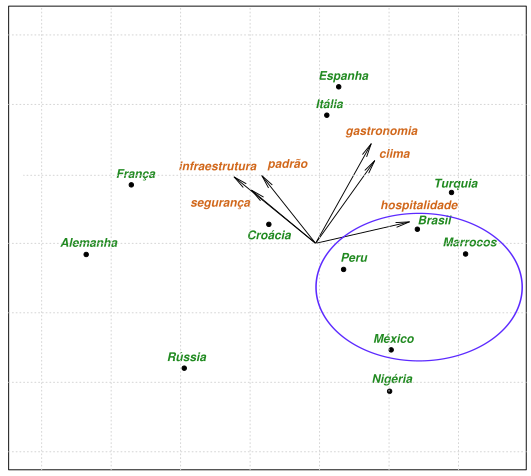
\includegraphics[width=\textwidth]{images/item-sel-orig.pdf}
    \caption{Interação do usuário.}
  \end{subfigure}%
  ~
  \begin{subfigure}[b]{0.45\textwidth}
    \centering
    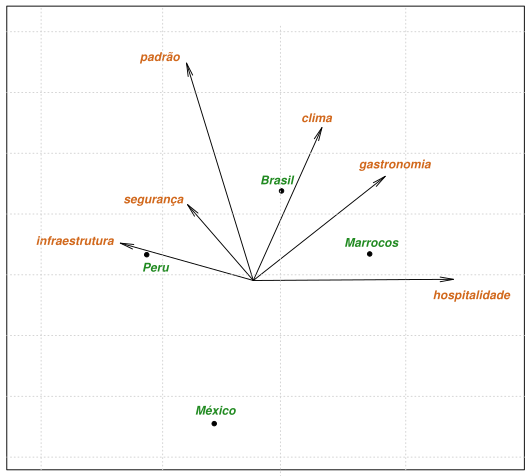
\includegraphics[width=\textwidth]{images/item-sel.pdf}
    \caption{Resultado esperado.}
  \end{subfigure} 
  \caption{Exemplo de seleção sobre itens.}
  \label{fig:item-sel}
\end{figure}

Nas seleções sobre dimensões pretende-se solucionar
basicamente dois problemas. O primeiro, chamado de mínimo
ótimo (\emph{minimal optimal})~\cite{Kohavi1997}, consiste
em construir um subconjunto dos atributos de entrada
evitando ao máximo a redundância entre eles. Um caso prático
deste problema está na construção de um classificador, onde
ao evitar redundância entre os atributos de entrada
pode-se fazer com que o método obtenha ganhos no tempo
de execução e na qualidade dos resultados. 

Já o segundo problema, conhecido como todos relevantes
(\emph{all relevant})~\cite{Nilsson2007}, equivale a
encontrar todos os atributos que são de algum modo
relevantes para a compreensão do fenómeno observado. Uma
aplicação real deste problema pode ser encontrada no
contexto de análise de expressões gênicas, onde deseja-se
identificar quais genes apresentam maior relação com o
diagnóstico de alguma doença. 

O uso de biplots permite que o usuário lide prontamente com
os dois problemas da seleção sobre dimensões. Em relação ao
primeiro problema, o usuário pode definir quais atributos
são redundantes ao observar as direções dos eixos. Assim,
quanto menor o ângulo entre dois eixos, maior é a correlação
entre eles e consequentemente maior a redundância. No
exemplo apresentado na Figura~\ref{fig:biplot}, observa-se
que os eixos correspondentes às variáveis infraestrutura e
segurança estão praticamente sobrepostos. Logo, o
usuário poderia descartar uma delas. 

Para lidar com o segundo problema, o usuário deve adotar 
algum eixo como referência. Como é exemplificado na
Figura~\ref{fig:item-sel}, o usuário poderia estar
interessado em investigar principalmente a infraestrutura
dos países. Assim, observaria que as variáveis gastronomia,
clima e hospitalidade são pouco relacionadas com esse
aspecto e poderia descartá-las. Ao realizar essa seleção o
usuário observaria uma nítida separação dos países europeus
e os restantes.

\begin{figure}[h!]
  \centering
  \begin{subfigure}[b]{0.45\textwidth}
    \centering
    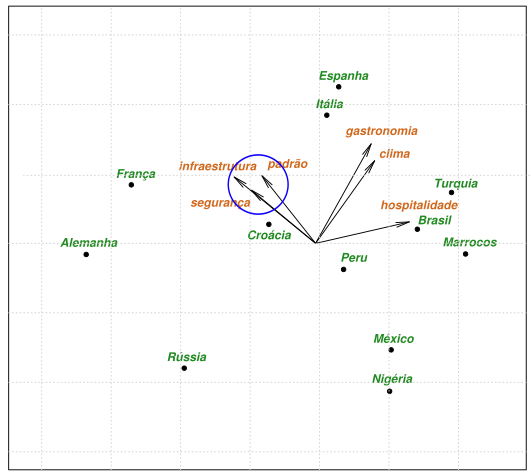
\includegraphics[width=\textwidth]{images/dim-sel-orig.pdf}
    \caption{Interação do usuário.}
  \end{subfigure}%
  ~
  \begin{subfigure}[b]{0.45\textwidth}
    \centering
    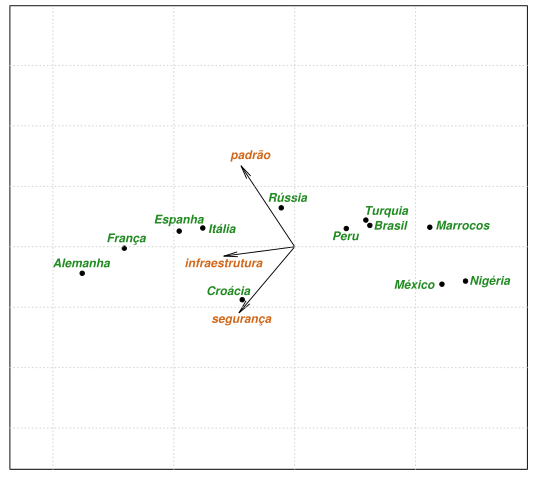
\includegraphics[width=\textwidth]{images/dim-sel.pdf}
    \caption{Resultado esperado.}
  \end{subfigure} 
  \caption{Exemplo de seleção sobre atributos.}
  \label{fig:item-sel}
\end{figure}

Existem situações onde somente o mecanismo de seleção sobre
dimensões não é suficiente para reduzir a redundância nos
dados. É o caso dos atributos gastronomia e clima do exemplo
apresentado. Nota-se que as duas variáveis apresentam certa
correlação. No entanto, o usuário pode ter dificuldade em
escolher qual das duas deve ser descartada. Para situações
como essa, propomos o uso do mecanismo de combinação de
atributos que é descrito a seguir.

\subsubsection{Mecanismo de Combinação de Atributos}

O mecanismo de combinação parte de um subconjunto de atributos
definido pelo usuário e retorna um único atributo que busca
representar o máximo da informação contida nesse subconjunto. A
Figura~\ref{fig:comb} ilustra uma combinação entre os atributos
gastronomia e clima. Espera-se que o eixo resultante possua 
direção semelhante aos que lhe deram origem e que as
características dos dados sejam preservadas.

\begin{figure}[h!]
  \centering
  \begin{subfigure}[b]{0.45\textwidth}
    \centering
    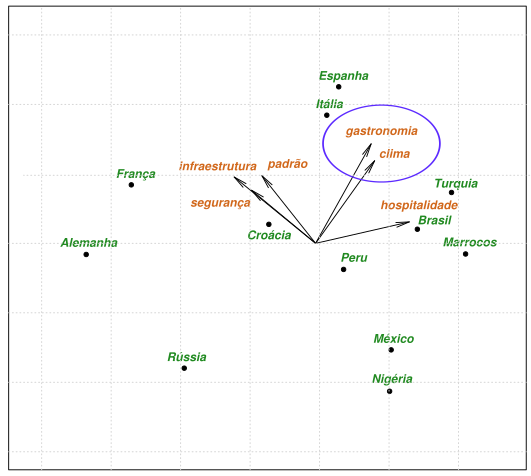
\includegraphics[width=\textwidth]{images/comb-orig.pdf}
    \caption{Interação do usuário.}
  \end{subfigure}%
  ~
  \begin{subfigure}[b]{0.45\textwidth}
    \centering
    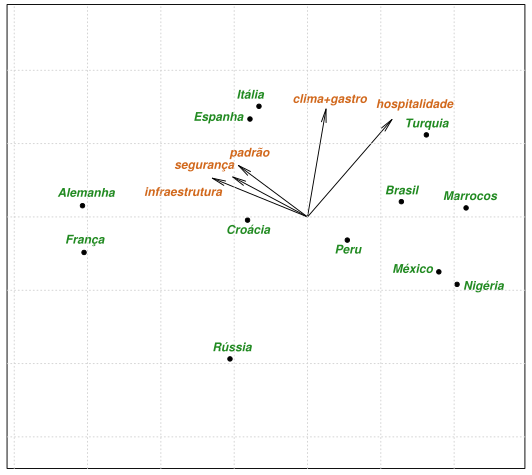
\includegraphics[width=\textwidth]{images/comb.pdf}
    \caption{Resultado esperado.}
  \end{subfigure} 
  \caption{Exemplo de combinação de atributos.}
  \label{fig:comb}
\end{figure}

Como o processo de combinação depende de métodos automáticos
como PCA, em certas situações esse mecanismo pode ser menos
intuitivo ao usuário do que o de seleção de atributos. No
entanto, em casos onde as dimensões dos dados não apresentam
um significado para o usuário, o mecanismo de
combinação pode ser preferível, pois não exige que o usuário
decida quais atributos devem ser descartados.

Acreditamos que o uso concomitante dos mecanismos de seleção
e combinação seja suficiente para se reduzir
eficientemente a dimensionalidade dos conjuntos de dados.
Entretanto, este projeto se propõe ir além do processo de
redução ao permitir que o usuário agregue mais incisivamente
seu conhecimento nos dados por meio do mecanismo de
construção de atributos que é detalhado a seguir.

\subsubsection{Mecanismo de Construção de Atributos}

Existem trabalhos na literatura que são capazes de agregar
o conhecimento do usuário nos dados. No entanto, esses
trabalhos modificam todo o conjunto de dados original
no processo. O mecanismo que propomos busca conservar as dimensões
originais e utilizar atributos ``fantasmas'' para
representar o conhecimento do usuário.

A Figura~\ref{fig:constr} ilustra o mecanismo de construção.
Inicialmente, cria-se um atributo ``fantasma'' com valores
arbitrários. O usuário então modifica o posicionamento dos
itens, no caso os países, conforme julga pertinente. As
novas posições dos pontos são utilizadas para transformar o
atributo ``fantasma'' em uma nova dimensão. Essa nova
dimensão tem o papel de representar aspectos subjetivos do
problema em estudo que não são facilmente medidos ou
capturados nas etapas de coleta e armazenamento dos dados.
Com isso, espera-se que tarefas subjacentes sobre os dados
obtenham melhores resultados. 

\begin{figure}[h!]
  \centering
  \begin{subfigure}[b]{0.45\textwidth}
    \centering
    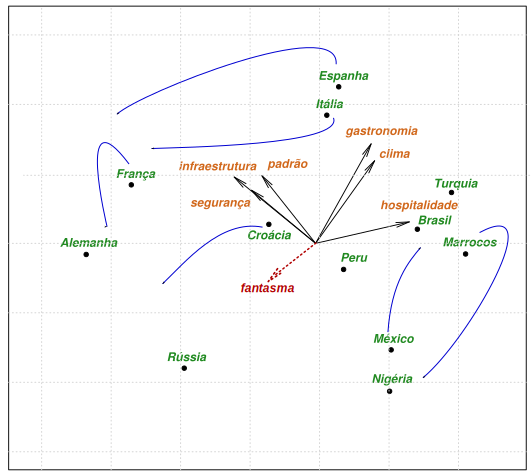
\includegraphics[width=\textwidth]{images/constr-orig.pdf}
    \caption{Interação do usuário.}
  \end{subfigure}%
  ~
  \begin{subfigure}[b]{0.45\textwidth}
    \centering
    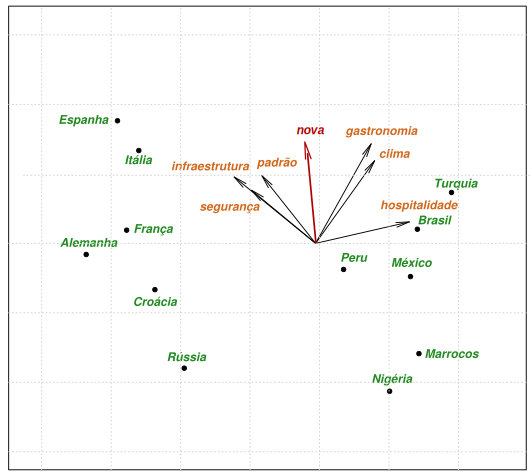
\includegraphics[width=\textwidth]{images/constr.pdf}
    \caption{Resultado esperado.}
  \end{subfigure} 
  \caption{Exemplo de construção de atributos.}
  \label{fig:constr}
\end{figure}

Como mencionado anteriormente, um aspecto importante de
ferramentas de visualização é a avaliação da incerteza dos
resultados. Como um biplot é também um mapeamento de
elementos no plano, ferramentas voltadas para esse tipo de
representação podem ser reaproveitadas, como
\emph{stress}~\cite{Kruskal1964}, \emph{Neighborhood
Hit}~\cite{Paulovich2008} e \emph{Neighborhood
Preservation}~\cite{Paulovich2008a}. Tais medidas
podem ser transmitidas nas representações visuais por meio
do uso de cores. Assim, durante todo o processo de
investigação e transformação dos dados, o usuário 
pode acompanhar a qualidade dos resultados apresentados. 

Dentre as possíveis aplicações para a ferramenta
desenvolvida, considera-se de grande relevância as
engajadas no contexto de recuperação de informação
(\emph{Information Retrieval})~\cite{Manning2008}.
Cogita-se, inclusive, o desenvolvimento de um protótipo de um
sistema de recomendação. O sistema consideraria
as interações do usuário para retornar recomendações mais
pertinentes. Acredita-se que as transformações serão de
grande valia, pois os interesses e preferências dos usuários
podem ser fatores subjetivos de difícil aquisição em etapas
de coleta de dados.

A seguir apresenta-se como será feita a análise e avaliação
dos resultados.

\section{Forma de Análise dos Resultados}

Com dados melhor representados, os métodos que operam sobre
eles, como classificadores e agrupadores de dados, devem
apresentar melhores resultados. Será justamente por meio de
uma quantificação dessa melhoria que será feita a validação
deste trabalho. A referência para se definir a qualidade dos
resultados será estabelecida com base em uma comparação com
métodos automáticos. 

Normalmente essas comparações são
feitas com base na taxa de acerto da classificação com os
dados originais e com os dados
transformados~\cite{Guyon2003,Joshi2007}. No entanto, devido
a heterogeneidade dos métodos de redução não é trivial
definir uma métrica única para as
avaliações~\cite{Medeiros2011}. Assim, considera-se também o
uso de medidas de avaliação de agrupadores de dados, como a
medida da Silhueta~\cite{Rousseeuw1987} e o Índice
Rand~\cite{Rand1971}.

Na próxima seção resume-se o que foi desenvolvido
até o momento da escrita deste documento. Isso inclui a
abordagem adotada antes da escolha de biplots como base para
as visualizações e também o arcabouço computacional da
ferramenta a ser desenvolvida.

\section{Resultados Preliminares}

A escolha de biplots como a visualização básica para este
projeto não foi uma decisão imediata. Inicialmente,
trabalhamos com visões coordenadas entre itens e
dimensões, algo como o apresentado na Figura~\ref{fig:dual}.
Para este exemplo utilizamos o conjunto de dados
Iris~\cite{Fisher1936} que possui 150 elementos e 5
atributos, sendo que um deles é a espécie das flores. Em
(a) temos a representação dos itens que pode ser construída
com base em qualquer técnica de redução de dimensionalidade
como PCA ou MDS. Enquanto em (b) apresenta-se a representação das
dimensões que demanda um processo de construção mais
elaborado. Em ambos casos a proximidade entre os
pontos é diretamente proporcional à similaridade dos
elementos que representam.

\begin{figure}[h!]
    \centering
    \begin{subfigure}[b]{0.45\textwidth}
        \begin{framed}
            \centering
            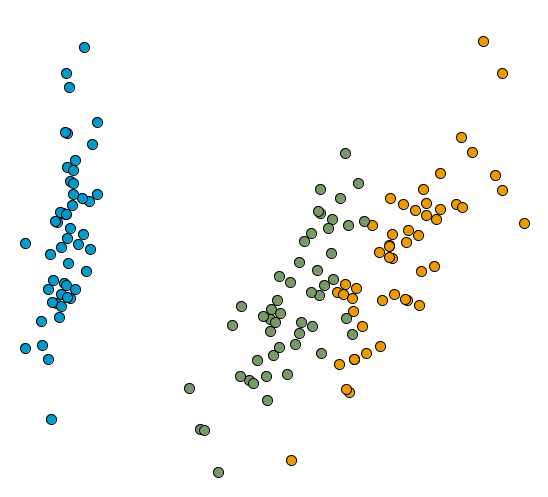
\includegraphics[width=\textwidth]{images/dual1.png}
        \end{framed}
        \caption{}
    \end{subfigure}%
    ~
    \begin{subfigure}[b]{0.45\textwidth}
        \begin{framed}
            \centering
            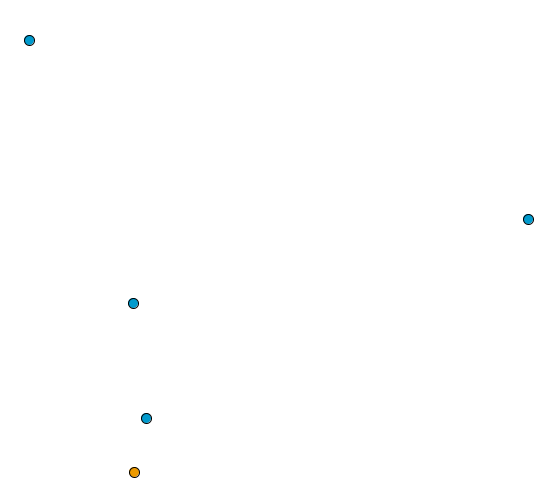
\includegraphics[width=\textwidth]{images/dual2.png}
        \end{framed}
        \caption{}
    \end{subfigure} 
    \caption{Exemplo da abordagem adotada inicialmente. Em
        (a) apresenta-se os itens com diferentes cores para
        flores de diferentes espécies. Em (b) apresenta-se
        as dimensões e destaca-se o atributo referente à
        espécie.}
    \label{fig:dual}
\end{figure}

O procedimento para a construção da representação das
dimensões é mais elaborado, pois envolve a difícil tarefa de
escolha de uma medida de similaridade entre atributos. De um
modo geral, uma medida de similaridade pode ser definida da
seguinte maneira: dado um conjunto de dados contendo $n$
elementos com $m-$dimensões, suas colunas podem ser
descritas por $m$ vetores $A_i(0\leq~i<m)$, cada uma
contendo $n$ números reais $a_{i,k},(0\leq~k<~n)$, uma
medida de similaridade $S$ deve retornar um número real
($S:\mathbb{R}^n\times \mathbb{R}^n\rightarrow\mathbb{R}$)
satisfazendo as seguintes condições:

\begin{enumerate}

    \item Positividade: $\forall A_i,A_j \in \mathbb{R}^n:
        S(A_i,A_j) \geq 0 $

    \item Reflexividade: $\forall A_i,A_j \in
        \mathbb{R}^n: (A_i = A_j) \Leftrightarrow
        S(A_i,A_j) = 0 $

    \item Simetria: $\forall A_i,A_j \in
        \mathbb{R}^n: S(A_i,A_j) =
        S(A_j,A_i)$, onde $(0 \leq i,j <
        d)$.

\end{enumerate}

A qualidade de uma medida de similaridade varia de
acordo com o domínio em que é aplicada. Normalmente, uma
medida é dita adequada quando há uma concordância entre o
valor obtido e a opinião de um especialista da área. No
entanto, mesmo um especialista em um assunto pode ter
dificuldade em determinar com precisão a semelhança entre
dois objetos. Assim, é muito difícil definir um modelo
matemático que meça a similaridade entre dois atributos com
precisão para todas as aplicações de forma genérica. 

A dificuldade em definir uma medida de similaridade é
somente um dos problemas dessa abordagem inicial.
Diferentemente do que acontece com biplots, a construção da
visualização apresentada na Figura~\ref{fig:dual} (b) exige
um processamento distinto do realizado para a
Figura~\ref{fig:dual} (a). Isso faz com que o custo
computacional seja praticamente duas vezes maior do que
utilizando-se biplots. Além disso, tal abordagem não
apresenta a coerência espacial entre o posicionamento dos
itens e das dimensões que os biplots oferecem.

Apesar de termos descartado essa abordagem inicial, grande
parte do que foi desenvolvido nessa etapa poderá ser
reaproveitado. Isso inclui a base da interface gráfica e
alguns dos mecanismos de interação. A
Figura~\ref{fig:dual-main} apresenta uma visão do geral do
protótipo desenvolvido. As janelas indicadas por (a) e (b)
correspondem às visualizações discutidas anteriormente.
Sobre essas visualizações já é possível selecionar
subconjuntos dos dados, tanto itens quanto dimensões. 

\begin{figure}[h!]
    \centering
    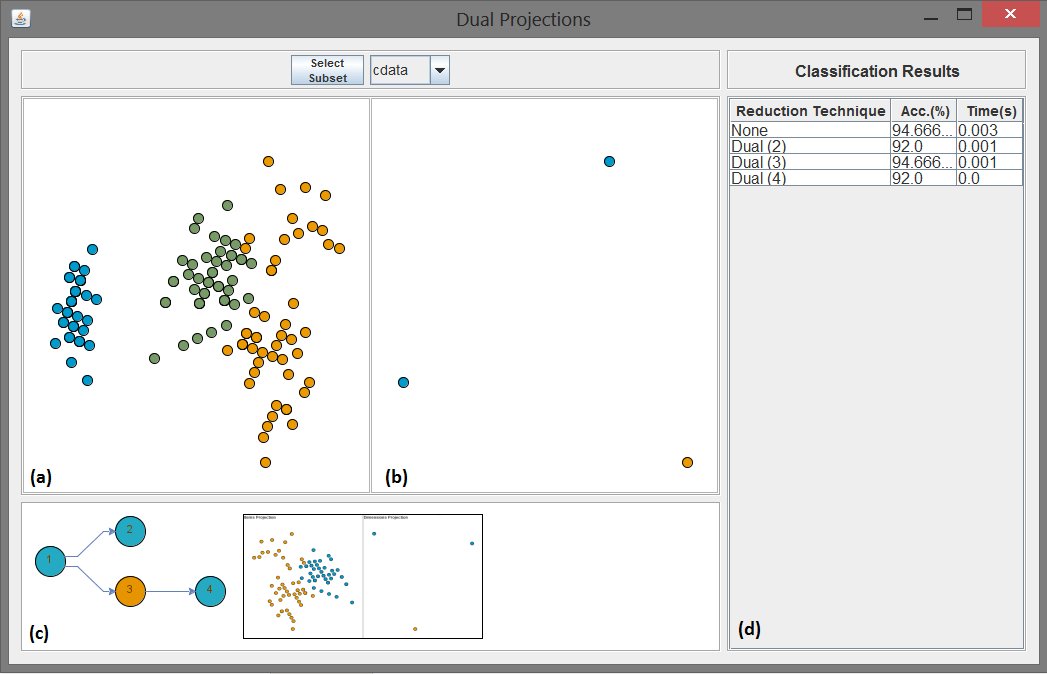
\includegraphics[width=16cm]{images/dual-main.png}
    \caption{Visão geral do protótipo desenvolvido.}
    \label{fig:dual-main}
\end{figure}

Ao interagir com os dados o usuário acaba modificando as
visualizações e pode perder o foco das análises. Buscando
amenizar esse problema, criamos a janela indicada por
(c), onde mantemos um histórico de todas as interações
realizadas pelo usuário. Exibimos esse histórico em uma
estrutura hierárquica e permitimos que o usuário interaja
com essa visualização para navegar em diferentes etapas das
investigações. 

Quando informações de classe são fornecidas, como por
exemplo o atributo espécie no caso do conjunto Iris, algumas
medidas para avaliação dos resultados são calculadas e
apresentadas na janela (d). Nesse protótipo inicial,
calculamos apenas a acurácia e o tempo de execução de um
classificador de dados. Porém, como já foi dito
anteriormente, adotaremos outras medidas, assim como outras
técnicas de transformação de dados multidimensionais para
realizar comparações. 

Tendo em vista o que já foi desenvolvido até o momento, a
seguir apresentamos as atividades que deverão ser executadas
para a conclusão deste trabalho de mestrado e o cronograma
no qual se encaixam.

\clearpage

\section{Plano de Atividades e Cronograma Previsto}\label{sec:cronograma}

As principais atividades deste trabalho de mestrado são as seguintes:

\begin{enumerate}
    \item Cumprimento das disciplinas da pós-graduação;

    \item Revisão bibliográfica;

    \item Implementação dos biplots como base da
        ferramenta visual;

    \item Desenvolvimento dos mecanismos de seleção e
        extração para redução interativa de
        dimensionalidade;

    \item Desenvolvimento do mecanismo de construção
        interativa de atributos;

    \item Desenvolvimento de um método para expressar
        a qualidade dos resultados apresentados;

    \item Implementação do protótipo de um sistema de
        recomendação;

    \item Avaliação dos resultados;

    \item Escrita e apresentação da dissertação para uma banca
        avaliadora. 
\end{enumerate}

O cronograma de execução das atividades é apresentado na Tabela~\ref{t:atividades}. 

\newcommand{\y}{\color{black}\rule{35pt}{7pt}}
\newcommand{\x}{\hspace*{35pt}}
\renewcommand{\r}{\color{cinza}\rule{35pt}{7pt}}
\setlength{\tabcolsep}{0pt}

\begin{table}[htb] 
\caption{Cronograma de Atividades.} 
\begin{center}
\begin{tabular}{|c|c|c|c|c|c|}
\cline{2-6}
\multicolumn{1}{l|}{} & \multicolumn{2}{c|}{2012} & \multicolumn{2}{c|}{2013} & \multicolumn{1}{c|}{2014} \\
    \hline \ Atividade\ \ 
    & 1\textordmasculine\ S. & 2\textordmasculine\ S. 
    & 1\textordmasculine\ S. & 2\textordmasculine\ S. 
    & 1\textordmasculine\ S. \\
    \hline \hline                                        
    %     &       2012        &       2013         &       2014       \\
        1     &\y\y    &\y\y      &\x\x     &\x\x      &\x\x     \\ \hline
        2     &\x\x    &\y\y      &\y\y     &\r\r      &\r\x     \\ \hline
        3     &\x\x    &\x\y      &\y\y     &\r\x      &\x\x     \\ \hline
        4     &\x\x    &\x\x      &\y\y     &\r\r      &\x\x     \\ \hline
        5     &\x\x    &\x\x      &\x\y     &\r\r      &\r\x     \\ \hline
        6     &\x\x    &\x\x      &\x\x     &\x\x      &\r\x     \\ \hline
        7     &\x\x    &\x\x      &\x\x     &\x\x      &\r\x     \\ \hline
        8     &\x\x    &\x\x      &\x\y     &\r\r      &\r\x     \\ \hline
        9     &\x\x    &\x\x      &\x\x     &\r\r      &\r\x     \\ \hline
        %     &       2012        &       2013         &       2014       \\
\end{tabular}
\end{center}
\label{t:atividades}
\end{table}
